\documentclass[a4paper, 12pt]{article}
\usepackage[T1]{fontenc}
\usepackage[utf8]{inputenc}
\usepackage{apacite}
\usepackage{mathptmx}
\usepackage{enumerate}
\usepackage[margin=0.5in]{geometry}
\usepackage{xspace}
\usepackage{tikz}
\usepackage{parskip} 


% chart attributes
\usetikzlibrary{shapes.geometric, arrows}
\tikzstyle{startstop} = [rectangle, rounded corners, minimum width=5cm, minimum height=1cm, text centered, draw=black, fill=green!30] %start
\tikzstyle{process} = [rectangle, minimum width=5cm, minimum height=1cm, text centered, draw=black, fill=blue!30] %process
\tikzstyle{arrow} = [thick,->,>=stealth] %arrow for chart

\renewcommand{\baselinestretch}{1.0}

\newcommand\nd{\textsuperscript{nd}\xspace}
\newcommand\rd{\textsuperscript{rd}\xspace}
\newcommand\nth{\textsuperscript{th}\xspace} %\th is taken already

\setlength\parindent{0pt} % set paragraph indent to zero

% fill up your name, ID, contribution and paper title here
\author{
LOA TAT ANN \quad 1221304731 \quad contribution1 \\
YU BUI XUAN \quad 241UC24121 \quad contribution2\\
MOHD SYAMEL BIN MOHD KARID \quad 1221309130 \quad contribution3\\
}
\title{ Optimizing DDoS Attack Detection with Machine Learning Algorithms and Multiple Datasets }

\begin{document}
\maketitle

%dataset size
%impact of datasets affecting the accuracy of machine learning DDoS detection methods (?)

\section*{Executive Summary}
%This includes the problem statement, objectives, research methodology, expected output and significance of output in a summary form. 

Distributed Denial-of-Service (DDoS) attacks have caused massive disruptions to network services, and they are difficult to detect as they blend in within normal traffic to evade detectors. Researchers have developed new methods such as machine learning to prevent threats from happening. Machine learning is prized for its good performance, but one of its key limitations for machine learning is a lack of suitable datasets and algorithms. The study aims to address dataset inadequacies and algorithm performance, which are some of the key challenges faced by researchers. Existing approaches used by researchers often get inaccurate results as most of them use outdated datasets or datasets with questionable quality. Besides that, each algorithm has its strengths and weaknesses. This study will assess the effectiveness of various techniques under diverse conditions by employing multiple datasets and a blend of ensemble methods to determine which methods are the most optimal for different tasks. The outcome of this research will be immense, as organizations can use the results to implement the solutions as practical applications and researchers can utilize the findings to augment further research and advancements in machine learning and cybersecurity. 

\textbf{Keywords:} \textit{research, cybersecurity, artificial intelligence, machine learning, ddos, ddos attacks, algorithms, dataset, optimization, ensemble}

\section{Introduction}
%This section contains a brief introduction to the research topic and background. \\
%Citation example: \citeA{1}

Distributed Denial-of-Service (DDoS) is a cyberattack method that utilizes multiple benign devices on a network and uses them to send malicious packets to disrupt networks with hopes of denying others normal access to them. DDoS attacks are difficult to detect, as they blend in with normal network traffic and use illegitimately obtained IP addresses to avoid being detected. \citeA{1} Because of this, it is hard to detect DDoS attacks which can cause massive damage to network infrastructure. Due to the increasing popularity of network technology, DDoS attacks are becoming more commonplace, as it was estimated that around 15.4 million DDoS attacks were recorded according to a report from Cisco. \citeA{10} 

With the threats of such attacks, various methods are developed to detect DDoS attacks and prevent them from happening. One of the methods proposed by researchers is machine learning detection, as they prize its performance and adaptability on such tasks. However, machine learning methods still have their issues, which include the fact that such methods may get varied results due to the varying quality and quantity of datasets and algorithms which are crucial to machine learning as they are used as a "guideline" to assist those algorithms to detect threats more accurately. As DDoS attacks evolve rapidly, current methods may not be capable of reacting to these new threats. \citeA{1}

In this research proposal, we will explore the methods to create a solution that optimizes machine learning on DDoS attack detection with the use of multiple algorithms and datasets. The research will comprehensively evaluate, compare and determine the best methods in a period spanning several years of research and development. We will also propose the related activities utilized in research, and get the expected results from there.

\section{Problem Statement}
We have identified that dataset and algorithm issues are some of the major reasons for inaccuracies in attack detection among machine learning. The dataset is a major part of machine learning detection as it uses the dataset to extract meaningful information to compare and detect similarities. Besides that, machine learning algorithms require the correct datasets to detect and treat the attack properly. \citeA{2} 

Studies have also stated that the lack of associated datasets and their features useful for cross-comparison is a major limitation of current research on machine learning in DDoS attack detection. \citeA{1} Also, not all datasets are comparable to each other, leading to data discrepancies. Besides that, most datasets used are either outdated, redundant or contain insufficient information. For instance, the CICDDoS2019 dataset only contains 1\% of benign records, with most records being hostile leading to an imbalance of data and bias in classification. \citeA{1} This could cause difficulty for machine learning algorithms when detecting traffic and potentially to accidentally classify benign traffic as a threat to the network, affecting real-time deployment. 

Researchers have proposed different methods to detect DDoS attacks, and there are differences in algorithms in various methods employed by the algorithms. Some methods such as SVM and Random Forest have good performance in detection while others have recorded weaker results. Researchers use different setups and methods to conduct experiments that could also affect results. \citeA{8} Application of such methods also varies depending of the algorithm, where some algorithms are harder to implement than others due to a complex structure. \cite{9} 

\clearpage

\section{Research Questions, Hypotheses and Objectives}
%Minimum of two and maximum of four for each of the research questions, hypotheses, and research objectives. You can use numbering/bullet point to list them out.

\subsection{Research Questions}
\begin{enumerate}
  \item How does dataset quality affect the accuracy of machine learning algorithms in DDoS attack detection?
  \item How do ensemble methods, which combine multiple machine learning algorithms compare to individual algorithms in terms of accuracy and robustness for DDoS attack detection? 
\end{enumerate}

\subsection{Hypotheses}
\begin{enumerate}
  \item The quality of datasets, which includes the completeness and relevance of data could significantly affect the accuracy of detecting DDoS attacks in IoT environments.
  \item Ensemble methods that combine multiple machine learning algorithms offer higher accuracy and robustness in DDoS attack detection compared to single algorithms.
\end{enumerate}

\subsection{Objectives}
\begin{enumerate}
  \item To evaluate the impact of dataset quality in the aspect of data completeness and relevance on the accuracy of DDoS attack detection.
  \item To prove the performance of ensemble methods is better than individual machine learning algorithms in terms of accuracy and robustness for DDoS attack detection. 
\end{enumerate}

\section{Literature Review Summary}

In the papers of Cheon, Ha, Lee, and Mun (2022), they approach DDoS detection with methods like Random Forests and Support Vector Machines which demonstrate high accuracy. However, their effectiveness is determined by the dataset's relevance and completeness. Using a poor-quality dataset can lead to an increasing number of false positives which could affect the reliability of these models.

Another issue involving datasets can be shown in the research by Esmaeili et al. (2022)
BiLSTM performs exceptionally well with an accuracy of 82.8\%, scoring the highest compared to other research methods. However, it could come with the risk of overfitting. This happens when the model is excessively trained using the NSL-KDD dataset which could result in difficulties. Furthermore, using the NSL-KDD dataset may not accurately reflect the nature of network traffic behaviour, which could impact the model's effectiveness, especially in real-life scenarios.

 Next, the use of an ensemble algorithm which is used in GRU-LM  and Word2vec architecture system as researched by Cheon et al. (2022), shows that the accuracy greatly improved compared to when using a single algorithm, as result shows that the integration of Word2vec and GRU-LM together could achieve the accuracy of 87.83\%, showcasing that the method achieved approximately 30\% higher than other types of models including RNN and LSTM. Cheon et al. (2022).

\clearpage

\section{Research Methodology}
%This section contains a description of the steps involved in research methodology, which also includes the metrics to be used for evaluating the proposed method along with a brief description of the techniques/models/methods/algorithms to be used.

\subsection{Overview}
The research methodology is structured into two main phases: data cleaning and segmentation, and third classification of such data using a neural network approach. These phases are conceived in a progressive process of pre-processing the dataset, mining the spatial features, and applying sophisticated machine learning algorithms for identifying and categorizing optical pathologic features such as vessels, disk optics, exudates and retinopatia cotton wool. The approach guarantees efficiency to increase the accuracy and reliability of the outcomes appropriate when dealing with difficult medical image data.

%You can use table/figure/image/graph in the report. All figures must have titles.

\subsection{ Selection and Training of Algorithms }

A selection of machine learning algorithms is chosen and planned to compare the performance of various algorithms in detecting DDoS attacks. Several algorithmic approaches, including K-Nearest Neighbors (KNN), Support Vector Machines (SVM), Naive Based Classifiers, Random Forest and others are selected, using relevant datasets like CCIDS2017 as a guideline for learning. \citeA{8} 

The training process of such algorithms is split into training and testing subsets, and each of the tests is recorded to extract important features such as packet size and traffic volume. The data are then compared with several metrics. The algorithms are compared by metrics such as accuracy, precision, and recall to determine which algorithm performed best on different conditions, and select the most effective algorithm from there.

\subsection{ Data Preprocessing Techniques }

This is to ensure that the dataset prepared is of the right quality and consistently processed to meet the intended model’s input standards. First, data cleaning removes the entries that are potentially less complete, which can lead to preconceptions during model training. When there are categorical variables without numerical values, the One-Hot Encoding is used that make the variables in the form of bit vectors, which is the most suitable for machine learning models. \citeA{8} Following this, normalization techniques including Min-Max scaling and Z-score normalization are performed. These methods come in handy in making the data look more standard and features are on a similar scale to enhance the training process in the model, thus avoiding large numbers influencing the training process. 

\subsection{ Image Segmentation and Feature Extraction }

This operation is of great importance in removing and distinguishing the regions of interest from the medical images which include blood vessels, optic discs, exudates, and cotton wool spots among others. Gaussian filtering applies methods where noise can be reduced and morphological operations that are useful in determining the outline of these characteristics \citeA{9}. This step brings down the number of variables making the next steps in the analysis much easier to carry out. In feature extraction, Random Forest technique and Principal Component Analysis (PCA) techniques are used to determine the features contributing towards the classification. This ensures that the model only centers all aspects to the data points that are exceptional thus improving the chances of the model in recognizing the abnormalities.

\subsection{ Classification Approach with Neural Networks }

The classification phase leverages neural networks, particularly LSTM networks, known for their ability to retain information over sequences, making them suitable for analyzing time-series data or complex image patterns \citeA{2}. These networks are trained with the selected features from the segmentation phase. The use of the ReLU (Rectified Linear Unit) activation function in hidden layers enables efficient learning, while advanced optimizers like Adam are employed to adjust the model weights iteratively, ensuring faster convergence during training. This step allows the model to learn complex relationships within the data, resulting in more accurate classification outcomes.

\subsection{ Model Evaluation Metrics }

For the performance examination of the proposed models, the following measures will be employed, accuracy, precision, recall and F1 score. Accuracy calculates the ratio of total instances that are predicted to be in one category out of total cases, and precision quantifies how many of the total instances identified to be in one specific category are actually in that category. Recall checks how well the model ‘catches’ all cases related to the category while the F1 score has the best characteristics when calculating the ratio between the number of true positives and both true and false positives and is highly suitable when working with imbalanced datasets \citeA{8}. They provide a full-scale assessment, and it is safe to assume that the chosen model is not only precise but also consistent in identifying anomalies.

\subsection{ Comparative Analysis of Classifiers }

This study explores many other classifiers such as Support Vector Machines (SVM), K-Nearest Neighbors (KNN), Random Forest, and Logistic Regression compared with neural networks \citeA{8}. Every algorithm is then compared in terms of certain criteria they provide, including accuracy, precision, recall and required computational time. This comparative analysis will help to define what pros and cons of each model exist, which in turn makes it easy to choose the proper algorithm for the task. The hope of achieving this is through comparing these models to the neural networks; thus, the kind of approach chosen meets the requisite efficiency and reliability in the classification of abnormalities in medical images.

This research approach guarantees the thorough and strategic approach of data pre-processing, feature selection/extraction, model training and testing processes by enhancing the robustness of the solution.

\clearpage

\section{Research Activities and Milestones}

\subsection{Flowchart for Activities}

Figure \ref{graph:1} is a flow chart showing the procedures that would be involved in the research. 
%Flowchart
\begin{figure}[ht]
    \centering
    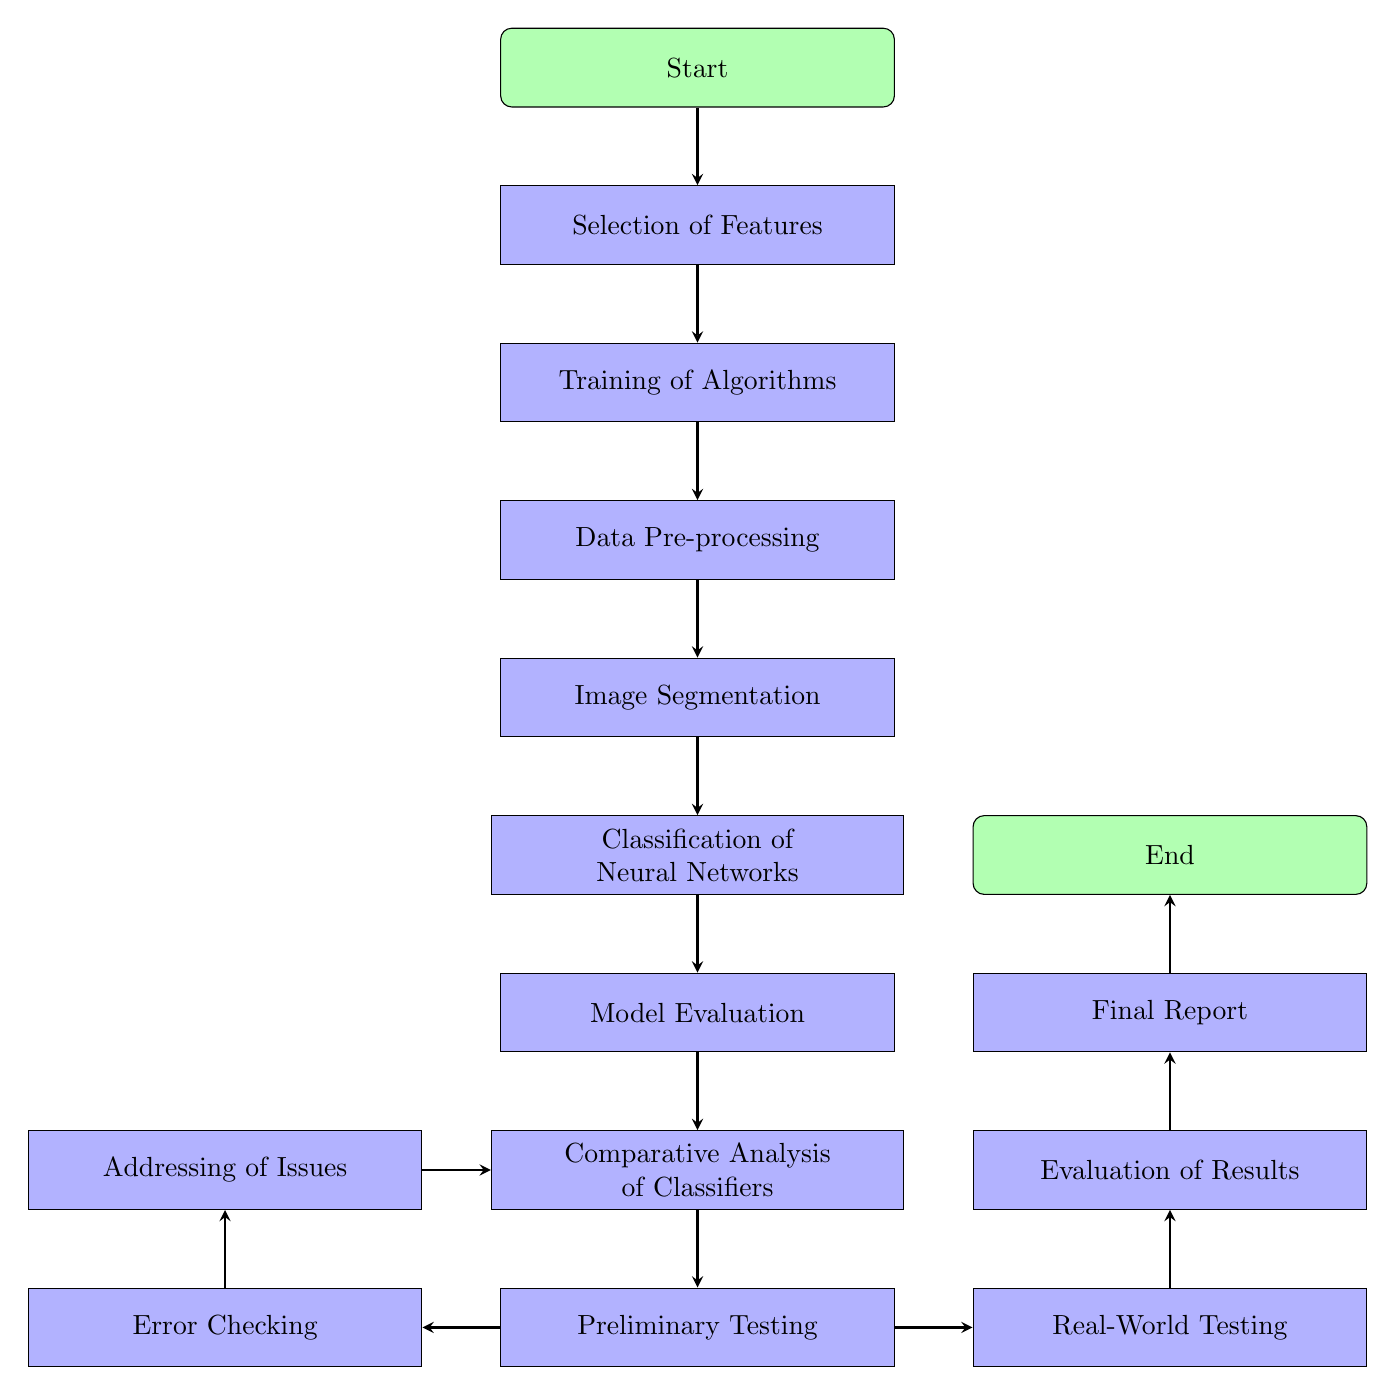
\begin{tikzpicture}[node distance=2cm]
    %nodes
    \node (start) [startstop] {Start};
    \node (proc) [process, below of=start] {Selection of Features};
    \node (proc1) [process, below of=proc] {Training of Algorithms};
    \node (proc2) [process, below of=proc1] {Data Pre-processing};
    \node (proc3) [process, below of=proc2] {Image Segmentation};
    \node (proc4) [process, below of=proc3] {\parbox{5cm}{\centering Classification of\\Neural Networks}};
    \node (proc5) [process, below of=proc4] {Model Evaluation};
    \node (proc6) [process, below of=proc5] {\parbox{5cm}{\centering Comparative Analysis\\of Classifiers}};
    \node (proc7) [process, below of=proc6] { Preliminary Testing };
    \node (proc7a) [process, left of=proc7, xshift=-4cm] { Error Checking };
    \node (proc7b) [process, above of=proc7a] { Addressing of Issues };
    \node (proc8) [process, right of=proc7, xshift=4cm] {Real-World Testing};
    \node (proc9) [process, above of=proc8] {Evaluation of Results};
    \node (proc10) [process, above of=proc9] {Final Report};
    \node (stop) [startstop, above of=proc10] {End};

    %arrows
    \draw [arrow] (start) -- (proc);
    \draw [arrow] (proc) -- (proc1);
    \draw [arrow] (proc1) -- (proc2);
    \draw [arrow] (proc2) -- (proc3);
    \draw [arrow] (proc3) -- (proc4);
    \draw [arrow] (proc4) -- (proc5);
    \draw [arrow] (proc5) -- (proc6);
    \draw [arrow] (proc6) -- (proc7);

    \draw [arrow] (proc7) -- (proc7a);
    \draw [arrow] (proc7a) -- (proc7b);
    \draw [arrow] (proc7b) -- (proc6);

    \draw [arrow] (proc7) -- (proc8);
    \draw [arrow] (proc8) -- (proc9);
    \draw [arrow] (proc9) -- (proc10);
    \draw [arrow] (proc10) -- (stop);
    
    \end{tikzpicture}
    \caption{Flow chart for the research.}
    \label{graph:1}
\end{figure}

\clearpage

\subsection{Activities Gantt Chart}
Figure \ref{gantt:1} and Table \ref{table:1} is a Gantt chart showing how long the research will be conducted and the time details about the research methods.

\begin{figure}[!ht]
    \centering
    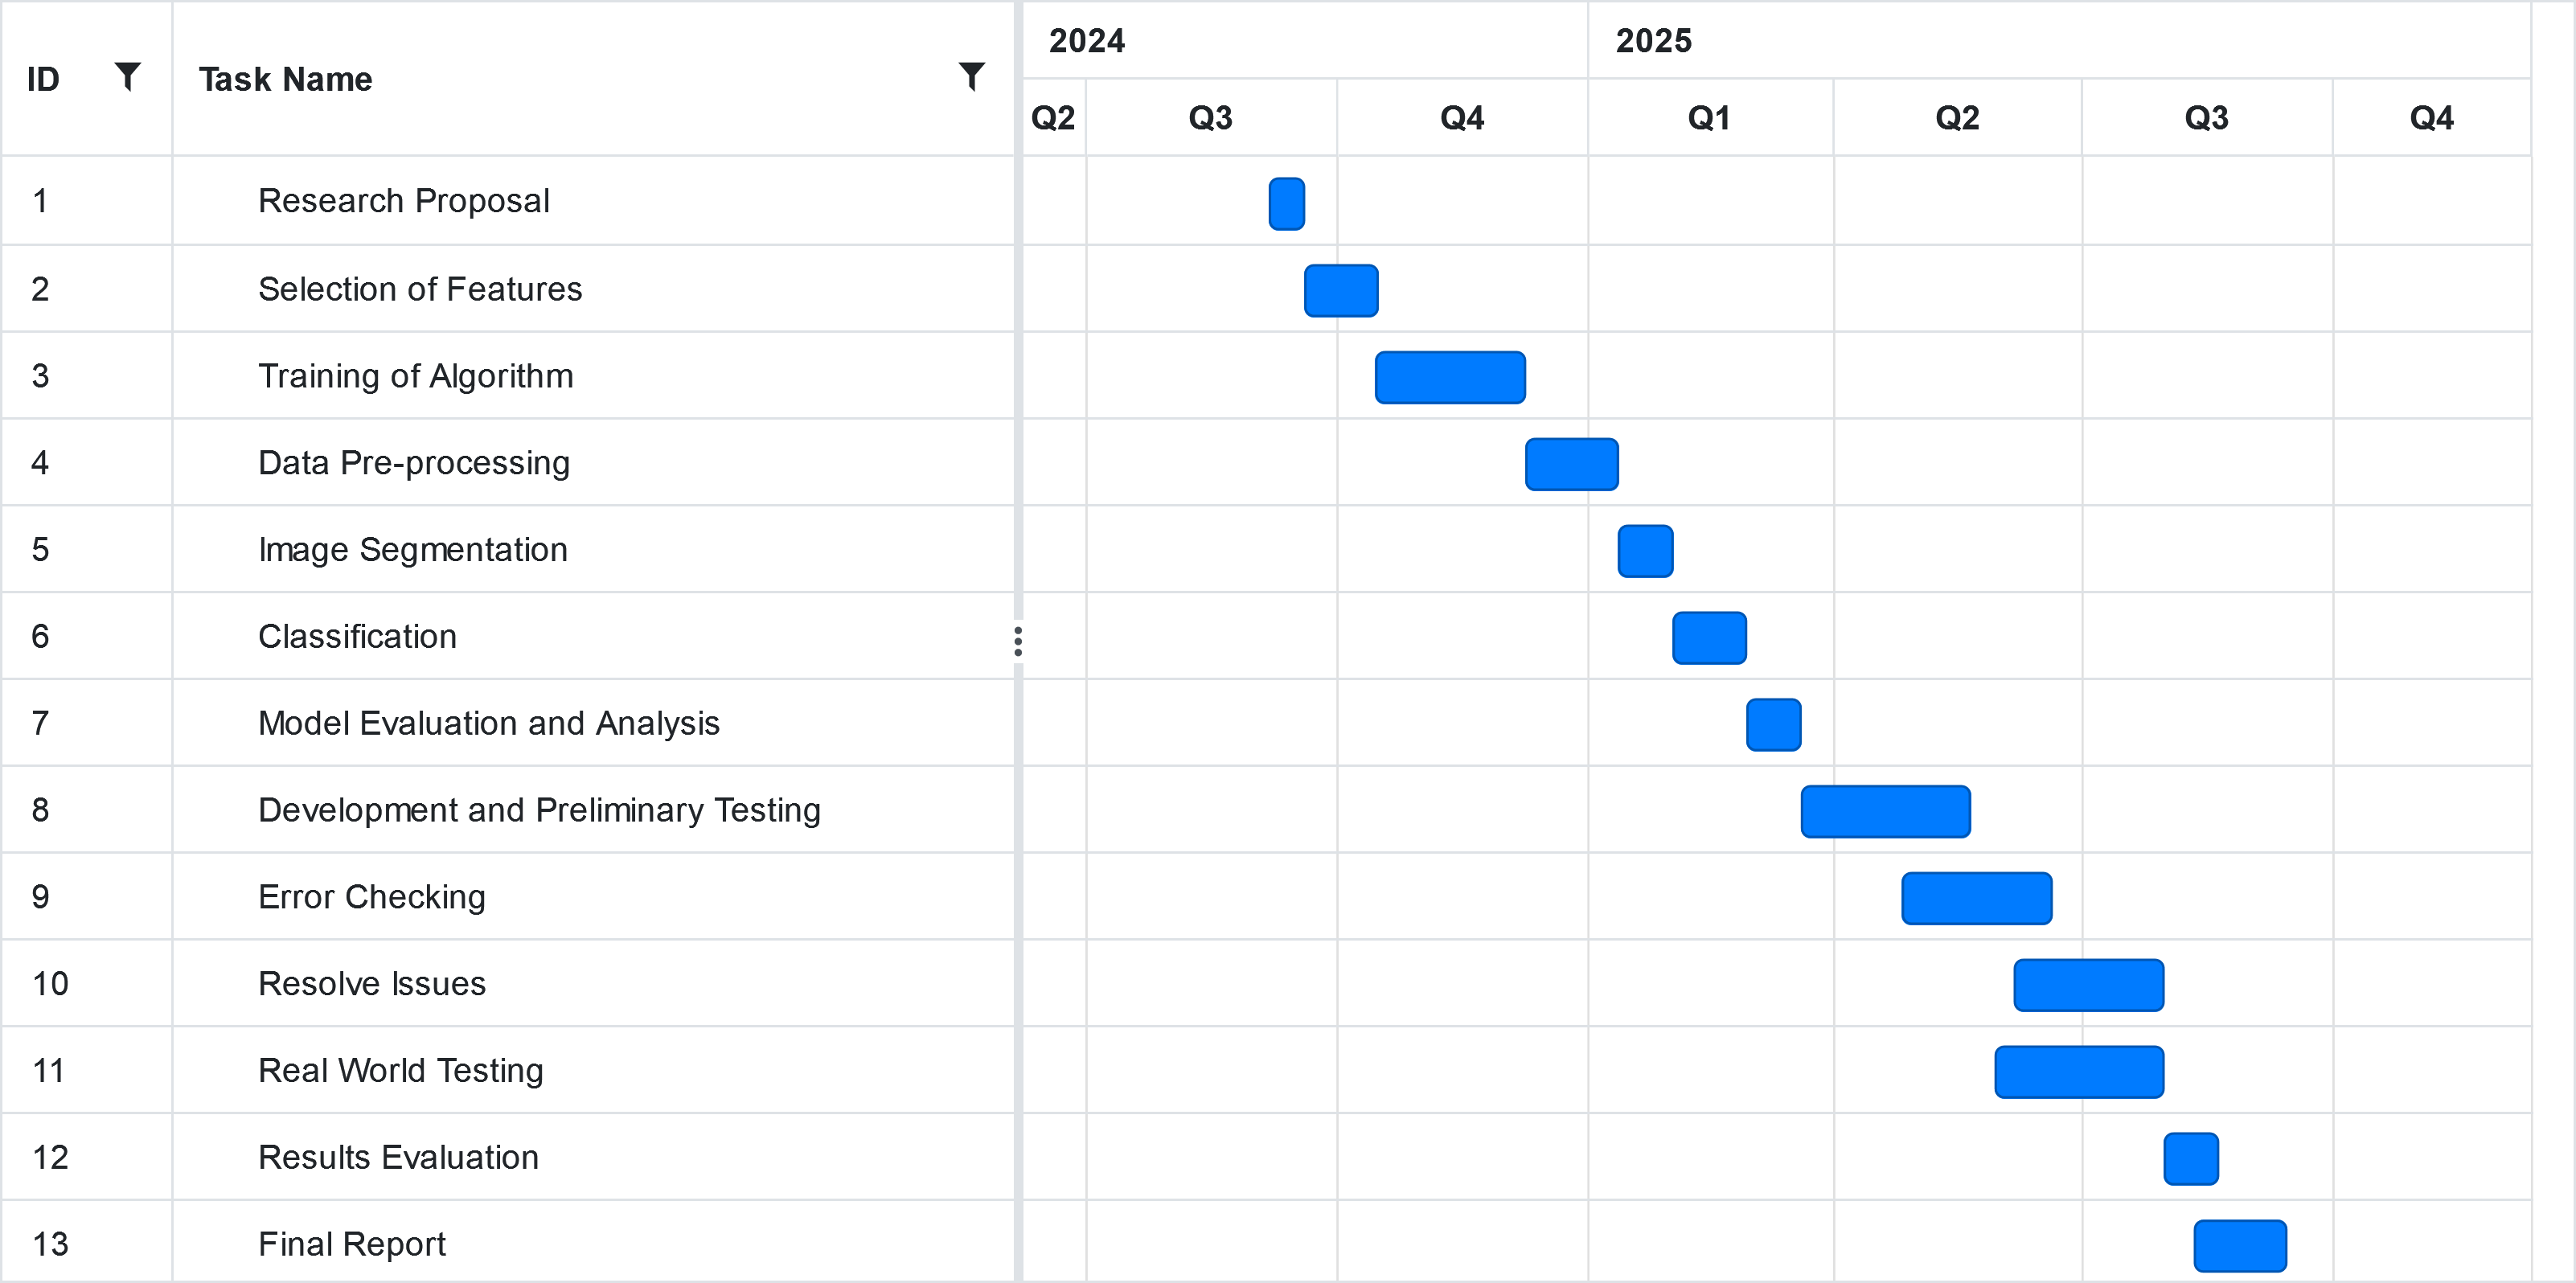
\includegraphics[width=1\linewidth]{gantt.png}
    \caption{Gantt Chart}
    \label{gantt:1}
\end{figure}

\begin{table}[!ht]
    \centering
    \begin{tabular}{|l|c|c|c|}
    \hline
        \textbf{Name} & \textbf{Start} & \textbf{Finish} & \textbf{Duration} \\ \hline
        \textbf{Research Proposal} & 2024-09-05 & 2024-09-18 & 14 days \\ \hline
        \textbf{Selection of Features } & 2024-09-18 & 2024-10-15 & 28 days \\ \hline
        \textbf{Training of Algorithm} & 2024-10-14 & 2024-12-08 & 56 days \\ \hline
        \textbf{Data Pre-processing} & 2024-12-08 & 2025-01-11 & 35 days \\ \hline
        \textbf{Image Segmentation} & 2025-01-11 & 2025-01-31 & 21 days \\ \hline
        \textbf{Classification} & 2025-01-31 & 2025-02-27 & 28 days \\ \hline
        \textbf{Model Evaluation} & 2025-02-27 & 2025-03-19 & 21 days \\ \hline
        \textbf{Preliminary Testing} & 2025-03-19 & 2025-05-20 & 63 days \\ \hline
        \textbf{Error Checking} & 2025-04-25 & 2025-06-19 & 56 days \\ \hline
        \textbf{Resolve Issues} & 2025-06-05 & 2025-07-30 & 56 days \\ \hline
        \textbf{Real World Testing} & 2025-05-29 & 2025-07-30 & 63 days \\ \hline
        \textbf{Results Evaluation} & 2025-07-30 & 2025-08-19 & 21 days \\ \hline
        \textbf{Final Report} & 2025-08-10 & 2025-09-13 & 35 days \\ \hline
    \end{tabular}
    \caption{Table of tasks involved}
    \label{table:1}
\end{table}

\clearpage

\section{Expected Results and Impact}

\subsection{Expected Results}
The main expected result of this research is the improvements in detection performance by selecting the best from multiple datasets and detection algorithms with a testing process. Besides that, we would also compare various algorithms to show other aspects of each algorithm and determine the best from them. By combining the data gathered we can optimize each setup for the most suitable task, enabling higher performance in DDoS attack detection. 

The results from the proposal could also be affected by real-time analysis of network traffic by gathering the results among multiple algorithms. It will also demonstrate its adaptability to various environments and tests can be scaled accordingly to counter various threats. 

\subsection{Expected Impact of Research}

\subsubsection{ Framework for Enhanced Cybersecurity Practices and Methods }

The proposed results can be used as part of an improved framework designed for real-time DDoS detection and prevention. Organizations can implement the framework in their network systems to improve their network security. The implementation of the system will lead to better adaptability against novel threats, improved operational stability, increased trust from customers and stakeholders, and compliance with national and state laws. 

\subsubsection{ Industry Adoption and Market Innovation }

Firms can adopt the methods and implement them in various practical applications. Such applications may include real-time network monitoring systems, customized detection frameworks and cyber threat intelligence platforms. The methods can also implemented within existing security systems to improve detection performance. With these implementations, innovators can drive innovation in the cybersecurity field by advancing the field with new ideas.

\subsubsection{ Foundation for Further Improvements and New Discoveries on the Field }

The resulting published work may also contribute to research efforts. The results may be published by reputable journals in the field, which could be used as a guideline for future research on the subject, enabling further improvements and new additions to improve the research quality of other journals. It can also be used as a baseline for research in other novel techniques and further advancements in machine learning and cybersecurity further down the line.

\clearpage

%References
\bibliographystyle{apacite}
\bibliography{MyBib}{}


\end{document}

